\documentclass[graphics]{beamer}

\usepackage{graphicx}
\usepackage{verbatim}
\usepackage{wrapfig}
\useoutertheme{shadow}
%\usecolortheme{orchid}
\usecolortheme{seahorse}


% math commands
\newcommand{\be}{\begin{eqnarray}}
\newcommand{\ee}{\end{eqnarray}}
\newcommand{\beq}{\begin{equation}}
\newcommand{\eeq}{\end{equation}}
\def\simless{\mathbin{\lower 3pt\hbox
      {$\rlap{\raise 5pt\hbox{$\char'074$}}\mathchar"7218$}}}
\def\simgreat{\mathbin{\lower 3pt\hbox
      {$\rlap{\raise 5pt\hbox{$\char'076$}}\mathchar"7218$}}} %> or of order

% variables

\def\toonscale{0.45}
\def\mboxy#1{\mbox{\small #1}}


\begin{comment}
\AtBeginSection[]{
  \frame{
    \frametitle{Outline}
    \tableofcontents[currentsection]
  }
}
\end{comment}

\title{Wave Optice lensing
}
%\subtitle{interim update}
\author[U. Pen]{Ue-Li Pen
\\ Dylan Jow, Job Feldbrugge, Neil Turok [8mm] 
}
\date{May 18, 2021}


\begin{document}

%\section*{Introduction}
\section{Lenses}

\begin{comment}
  \subsection{Outline}

  \frame{
    \frametitle{Outline}
    \tableofcontents
  }
\end{comment}

\frame{\maketitle}



  \frame{
    \frametitle{Lenses}
    \begin{itemize}
        \item Gravitational Lensing: micro, macro
        \item Plasma lensing
        \item Coherent sources: forms interference pattern
        \item expected (observed) for FRBs
        \item 
        \item 
        \item 
    \end{itemize}
  }


  \frame{
\vspace{-0.5in}
    \frametitle{History}
    \begin{itemize}
    \item Huygens, Fermat, 
    \item Picard-Lefschitz (19th century), Witten (2010)          
        \item concept: Oscillatory path integral
        \item 
        \item imaginary images
        \item 
            
    \end{itemize}
  }


  \frame{
\vspace{-0.5in}
    \frametitle{Optics: Geometric, Eikonal, Wave, P-L}
    \begin{itemize}
        \item Consider 1-D lens
        \item potential lensing function $\Psi(\theta)$
    \end{itemize}
\vspace{-1in}\hspace{2.5in}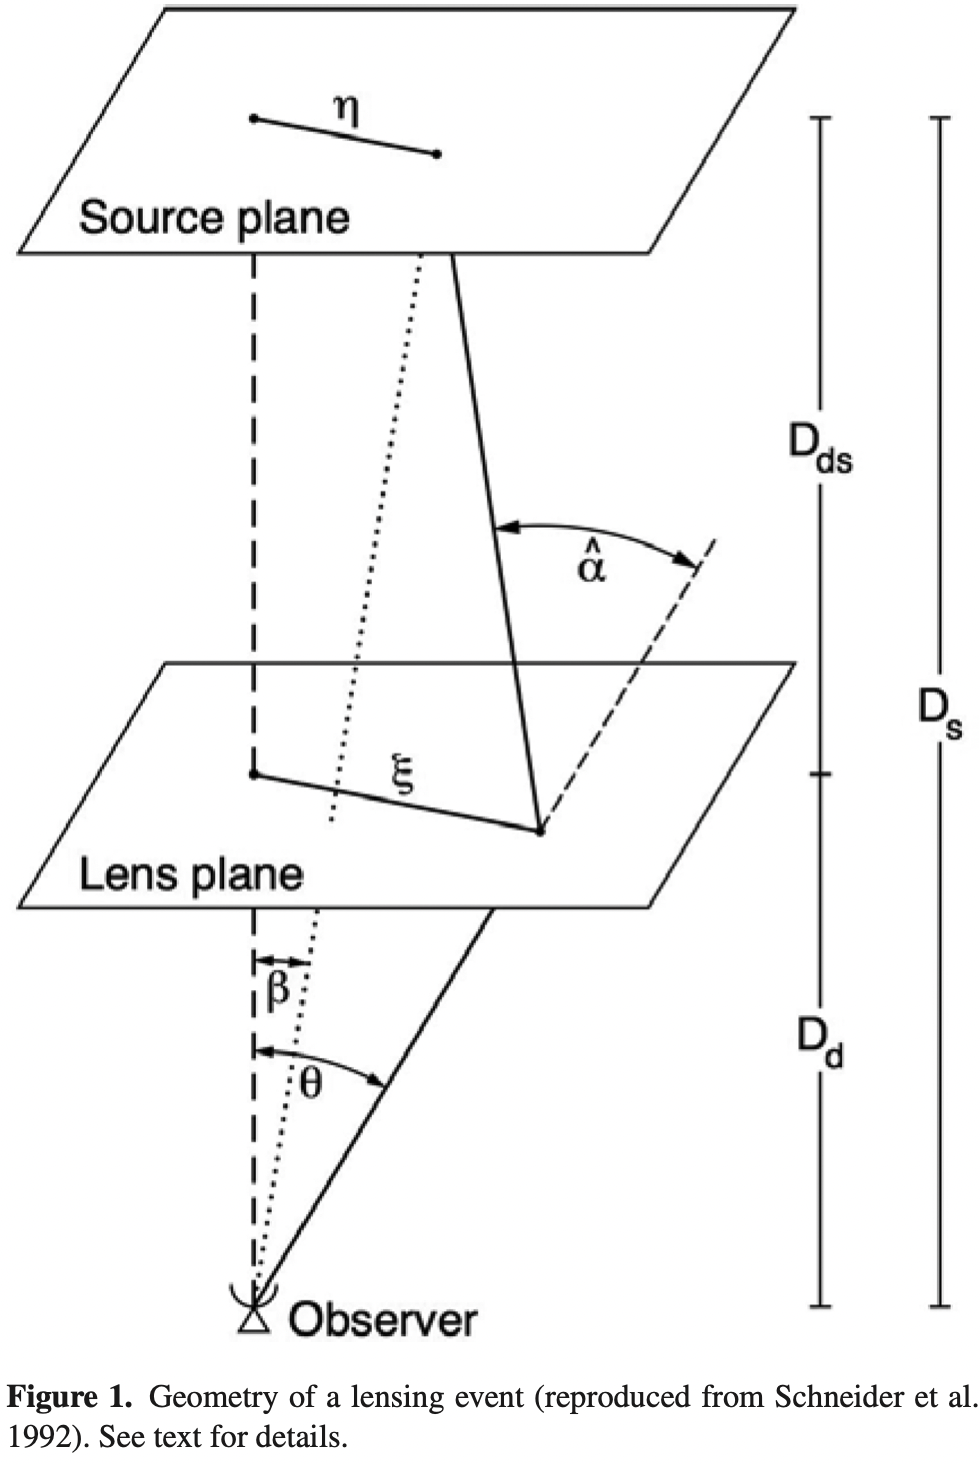
\includegraphics[width=1.5in]{Figures/lens.png}

  }

  \frame{
\vspace{-0.5in}
    \frametitle{New Observables}
    \begin{itemize}
    \item weak lensing: imaginary image allows time delay measurement
    \item strong lensing: delay measurements enable measurement of co-linearity
    \item microlensing: instant time delay, planets
    \item macrolensing: potentially nano-second delay -- universe expands!
    \item
    \item          
    \end{itemize}
  }
  \frame{
\vspace{-0.5in}
    \frametitle{Imaginary Images}
    \begin{itemize}
    \item consider ``rational lens'' potential $\psi(\theta)=\alpha/(1+x^2)$
    \item Geometric/eikonal images at $\psi'=x$
    \item 5 roots.  1 or 3 real roots, rest imaginary
    \item P-L: at most one imaginary image contributes!
    \item imaginary image can be brighter than unlensed real image
    \item 
    \end{itemize}
  }

  \frame{
\vspace{-0.5in}
    \frametitle{Microlensing}
    \begin{itemize}
    \item Jow+ 2020
    \item point lens
    \item Einstein radius $r_E^2=r_G D$
    \item Fresnel scale $r_F^2=\lambda D$
    \item 
    \item 
    \end{itemize}
  }

  \frame{
\vspace{-0.5in}
    \frametitle{Macrolensing}
    \begin{itemize}
    \item Wucknitz+ 2021
    \item alternate approach to cosmography
    \item triangulation: lens model+time delay measurement = $H_0$
    \item weak link has been lens model
    \item Wave optics: time delay observable to nanoseconds
    \item 
    \end{itemize}
  }

\end{document}
